\documentclass[14pt, a4paper]{extarticle}	
\usepackage{GOST}

\makeatletter
\renewcommand\@biblabel[1]{#1.}
\makeatother
\usepackage{longtable}

\graphicspath{{images/}}

\begin{document}
{ \begin{table}[ht]
	\centering
	\begin{tabular}{|c|p{400pt}|} 
	\hline
		\begin{tabular}[c]{@{}c@{}} 
\includegraphics[scale=0.8]{b_logo} \\\end{tabular} &
		\footnotesize\begin{tabular}[c]{@{}c@{}}\textbf{Министерство~науки~и~высшего~образования~Российской~Федерации}\\\textbf{Федеральное~государственное~бюджетное~образовательное~учреждение}\\\textbf{~высшего~образования}\\\textbf{«Московский~государственный~технический~университет}\\\textbf{имени~Н.Э.~Баумана}\\\textbf{(национальный~исследовательский~университет)»}\\\textbf{(МГТУ~им.~Н.Э.~Баумана)}\\\end{tabular}  \\
	\hline
	\end{tabular}
\end{table}
\noindent\rule{\textwidth}{4pt}
\noindent\rule[14pt]{\textwidth}{1pt}
\hfill 
\noindent
\makebox{ФАКУЛЬТЕТ~}%
\makebox[\textwidth][l]{\underline{~~~~~«Информатика и системы управления»~~~~~~~~~~~~~~~~~~~~~~~~~}}%
\\
\noindent
\makebox{КАФЕДРА~}%
\makebox[\textwidth][l]{\underline{«Программное обеспечение ЭВМ и информационные технологии»}}%

\begin{center}
	\vspace{1.5cm}
	{\bf\huge Расчетно-пояснительная записка\par}
	{\bf\Large к курсовой работе\par}
	\vspace{0cm}
\end{center}


\noindent
\makebox{\large{\bf Тема:}~~~}
\makebox[\textwidth][l]{\large\underline{~Разработка протокола с дедупликацией~~~~~~~~~~~~~}}\\

\noindent
\makebox{\large{\bf Дисциплина:}~~~}
\makebox[\textwidth][l]{\large\underline{~Компьютерные сети~~~~~~~~~~~~~~~~~~~~}}\\

\vspace{1cm}
\noindent
\begin{tabular}{l c c c c c}
    Студент      & ~ИУ7-75Б~       & \hspace{2.5cm} & \hspace{3cm}               & &  П.К Хетагуров \\\cline{2-2}\cline{4-4} \cline{6-6} 
    \hspace{3cm} & {\footnotesize(Группа)} &                & {\footnotesize(Подпись, дата)} & & {\footnotesize(И.О. Фамилия)}
\end{tabular}

\vspace{0.5cm}

\noindent
\begin{tabular}{l c c c c}
    Руководитель проекта & \hspace{3.3cm}   & \hspace{3.5cm}              & & Н.О. Рогозин \\\cline{3-3} \cline{5-5} 
    \hspace{2.9cm}  &              & {\footnotesize(Подпись, дата)} & & {\footnotesize(И.О. Фамилия)}
\end{tabular}

\begin{center}	
	\vfill
	\large \textit {Москва, 2021}
\end{center}

\thispagestyle {empty}
\pagebreak}
\setcounter{page}{3}

% СОДЕРЖАНИЕ 
\clearpage
\tableofcontents

\clearpage
\section*{Введение}
\addcontentsline{toc}{section}{Введение}
	Современные вычислительные системы сложно представить без поддержки интернет-сетей. Сети являются основным средством передачи информации. От качества соединения зависит работа большого количества сервисов и учереждений.\\
\indent Основными проблемами, влияющими на качество связи являются следующие:
\begin{itemize}
	\item высокий RTT(round-trip-time)\cite{quality};
	\item высокий процент потерь пакетов;
	\item получение пакетов в порядке, отличном от порядка отправки;
	\item дублирование пакетов.
\end{itemize}
\indent В данной работе будет рассмотренна проблема дублирования пакетов.

\clearpage
\section{Аналитический раздел}
\subsection{Постановка задачи}
В соответствии с заданием на курсовую работу необходимо разработать и реализовать метод определения и отбрасывания дубликатов пакетов. \\
\indent Для достижения цели курсовой работы необходимо решить следующие задачи:
\begin{itemize}
	\item проанализировать существующие методы решения;
	\item спроектировать протокол;
	\item реализовать спроектированный протокол;
	\item протестировать реализованный протокол.
\end{itemize}
\indent Разрабатываемый протокол должен отбрасывать дубликаты уже пришедших пакетов.


\subsection{Общие сведения}
Канал обычно характеризуются следующими характеристикам:
\begin{enumerate}
	\item RTT (Round Trip Time). Представляет собой время между отправкой запроса и получением ответа. На RTT влияет как физические ограничения скорости передачи 	сигнала в зависимости от среды (медь, оптоволокно, радиосигнал) и расстояния, так и ограничения в скорости обработки трафика в промежуточных узлах;
	\item bandwidth. Ширина канала - максимально возможное количество данных, которые могут быть переданы через канал за некоторый промежуток времени;
	\item lossrate (процент потерь пакетов).
\end{enumerate}
\indent \indent Вышеприведенные характеристики и вытекающие из них используются не только для общей оценки качества канала, но и в прикладных алгоритмах для его улучшения.

\subsection{Анализ существующих решений}
Уровень, который интересует нас на модели OSI - четвертый (транспортный). \\
Рассмотрим некоторые протоколы транспортного уровня.

\subsubsection{UDP}
User Datagram Protocol (UDP) - один из базовых протоколов сети. Протокол быстр, не гарантирует, что пакеты будут доставлены в том порядке, в котором они были отправлены и даже сам факт доставки. В протоколе отсутствуют пакеты подтверждения. Не требует открытия соеденения, пакеты отправляются сразу по готовности.\\
\indent  UDP используется когда требуется скорость доставки, а гарантией и правильностью доставки можно пренебречь, а также для широковещательной передачи. Протокол UDP определен в RFC 786\cite{rfc768}.

\subsubsection{TCP}
Transmission Control Protocol (TCP) - второй базовый протокол транспортного уровня. Гарантирует надежную доставку пакетов в определенном порядке. Использует пакеты подтверждения и повторную отправку пакета в случае его утери или искажения. Соединение должно установиться до начала передачи данных. \\ 
\indent TCP медленный, так как использует механизм контроля получения пакетов, что требует больших затрат времени. Используется в случаях, требующих надежную доставку сообщений. Протокол TCP определен в \text{RFC 793\cite{rfc793}.} \\
\indent Протокол TCP, в отличии от UDP использует метрики, собираемые в процессе работы протокола, для определения дальнейшей работы. Из полученных метрик высчитывается размер TCP окна, показывающий количество байт, которыепринимающая сторона готова принять в текущий момент без подтверждения. \\ 
\indent Помимо RTT и lossrate TCP вводит понятие отклонения RTT (devRTT). DevRTT и средний RTT используется для определения промежутка времени, после которого пакеты будут считаться утерянными в случае отсутствия подтверждающих пакетов. Далее приводятся формулы, которым оперирует TCP.
\begin{equation}
	RTT_{i} = t_{r} - t_{0} \text{,}
\end{equation}
\begin{tabular}{rl}
	где & $t_{r}$ - время получения подтверждающего пакета; \\
	& $t_{0}$ - время отправки пакета; \\
	& $RTT_{i}$ - RTT i-ого пакета. 
\end{tabular}

\begin{equation}
	RTT_{average}= \alpha RTT_{average} + \beta{RTT_{i}} \text{ ,}
\end{equation}
\begin{tabular}{rl}
	где & $RTT_{average}$ - среднее RTT; \\
	& обычно $\alpha$ = 0,875, $\beta$ = 0,125.
\end{tabular}

\begin{equation}
	dev_{i} = | RTT_{i} - RTT_{average} |\text{ ,}
\end{equation}
\begin{tabular}{rl}
	где & $dev_{i}$ - devRTT i-ого пакета.
\end{tabular}

\begin{equation}
	dev_{average} =\alpha dev_{average} + \beta{dev_{i}} \text{ ,} 
\end{equation}
\begin{tabular}{rl}
	где & $dev_{average}$ - среднее devRTT; \\
	& обычно $\alpha$ = 0,75, $\beta$ = 0,25.
\end{tabular}

\begin{equation}
	timeout =  RTT_{average} + 4 dev_{average}
\end{equation}

Заголовок\cite{tcpheader} TCP пакетов представлен на рисунке \ref{tcp-header}.
\begin{figure}[H]
	\centering
	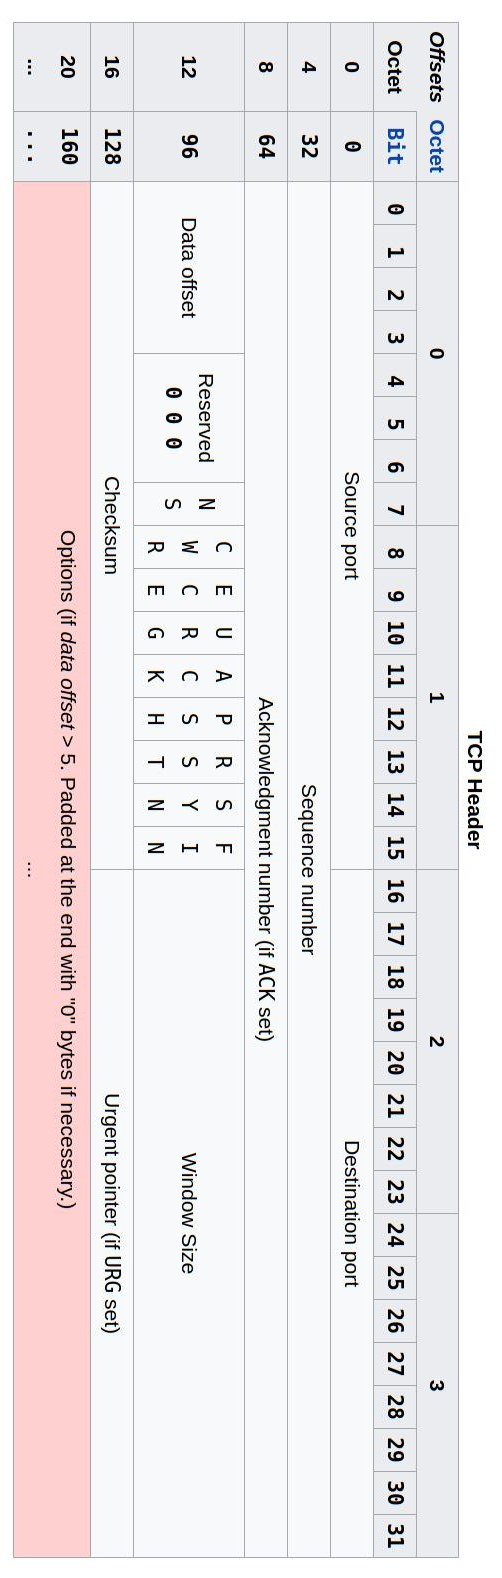
\includegraphics[scale=0.6]{tcpheader.jpg}
	\caption{Заголовок TCP пакета}
	\label{tcp-header}
\end{figure}

Расшифровка полей:
\begin{longtable}[H]{ |p{3cm} |p{3cm}| p{8.5cm} |}
	\caption{Расшифровка полей заголовка TCP пакета.}
	\hline
	Поле & Длина & Описание \\ \hline 
	\endfirsthead
	\hline
	Поле & Длина & Описание \\ \hline 
	\endhead
	\hline
	\multicolumn{3}{r} пПродолжение на следующей странице$\ldots$
	\endfoot
	\hline 
	\endlastfoot
	
	Порт источника & 2 байта & Номер порта источника \\ \hline 
	Порт назначения  & 2 байта & Номер порта назначения \\ \hline 
	Последова- тельный номер & 4 байта & Последовательный номер генерируется источником и используется назначением, чтобы переупорядочить пакеты для создания исходного сообщения и отправить подтверждение источнику. \\ \hline
	Номер подтверждения & 4 байта & Если установлен бит АСК поля "Управление", в данном поле содержится следующий ожидаемый последовательный номер. \\ \hline 
	Смещение данных & 4 байта & Информация о начале пакета данных. \\ \hline 
	Резерв & 6 битов & Резервируются для будущего использования \\ \hline 
	Управление & 6 битов & Биты управления содержат флаги, указывающие, верны ли поля подтверждения (АСК), указателя срочности (URG), следует ли сбрасывать соединение (RST), послан ли синхронизирующий последовательный номер (SYN) и т. д. \\ \hline
	
	Размер окна & 2 байта & В этом поле указывается размер приемного буфера. Используя подтверждающие сообщения, получатель может информировать отправителя о максимальном размере данных, которые тот может отправить. \\ \hline 
	Контрольная сумма & 2 байта & Контрольная сумма заголовка и данных; по ней определяется, был ли искажен пакет \\ \hline 
	Указатель срочности & 2 байта & В этом поле целевое устройство получает информацию о срочности данных. \\ \hline 
	Опции & переменная &  Необязательные значения, которые указываются при необходимости \\ \hline
	Дополнение & переменная & В поле дополнения добавляется столько нулей, чтобы заголовок заканчивался на 32-битной границе \\ \hline 
\end{longtable}

В алгоритме TCP алгоритм отбрасывания пакетов, приходящих вне своей очереди или дублированных, реализован с помощью сравнения поля с последовательным номером пакета с текущим TCP-окном. В самом тривиальном случае, если номер пакета больше или меньше крайних значений TCP порта, пакет отбрасывается. Если номер пакета находится внутри текущего окна и ещё не пришел, то его номер сохраняется и происходит принятие пакета. Если же номер уже существует, то пакет отбрасывается как дублированный.

\subsection{Вывод}
В аналитической части были проанализированы два основных сетевых протокола транспортного уровня (TCP и UDP), были разобраны особенности протокола TCP. \\
\indent На основании проведенного анализа можно сделать вывод, что свой протокол необходимо реализовывать на основе протокола UDP и алгоритма отбрасывания пакета в TCP.

\clearpage
\section{Конструкторский раздел}
В данном разделе будут спроектирован и описан разрабатываемый протокол.
\subsection{Проектирование протокола}
Из аналитической части стало понятно, что для определения дублированных пакетов необходимо ввести как минимум уникальный идентификатор пакета. Таким образом добавляется заголовок, содержащий метаинформацию. \\
\indent На принимающей стороне необходимо обеспечить хранение номеров принятых пакетов. Это можно сделать различными способами. \\
\indent Первый способ --- хранить номера пакетов отдельно, с помощью массива, списка или хэш-таблицы. У этого способа есть как плюсы так и минусы. \\
\indent Плюсы:
\begin{enumerate}
	\item простота хранения и доступа к номеру пакета;
	\item простота добавления новых номеров пакета.
\end{enumerate}
\indent Главным минусом же является большое количество памяти, затрачиваемое на хранение номеров. \\
\indent Второй способ предполагает групировку пакетов набором диапазонов. В этом методе номера 1, 2, 3...10 хранятся не по отдельности а в виде двух чисел --- началу и конец диапазона (1, 10). \\
\indent Плюсом такого подхода является намного меньший объем занимаемой памяти, а главным минусом --- сложность в добавлении нового номера пакета к существующим диапазонам. \\
\indent Для реализации был выбран второй подход. На рисунках \ref{check1}--\ref{check3} представлена схема алгоритма проверки вхождения и добавления номера пакета в существующий набор диапазонов.

\begin{figure}[H]
	\centering
	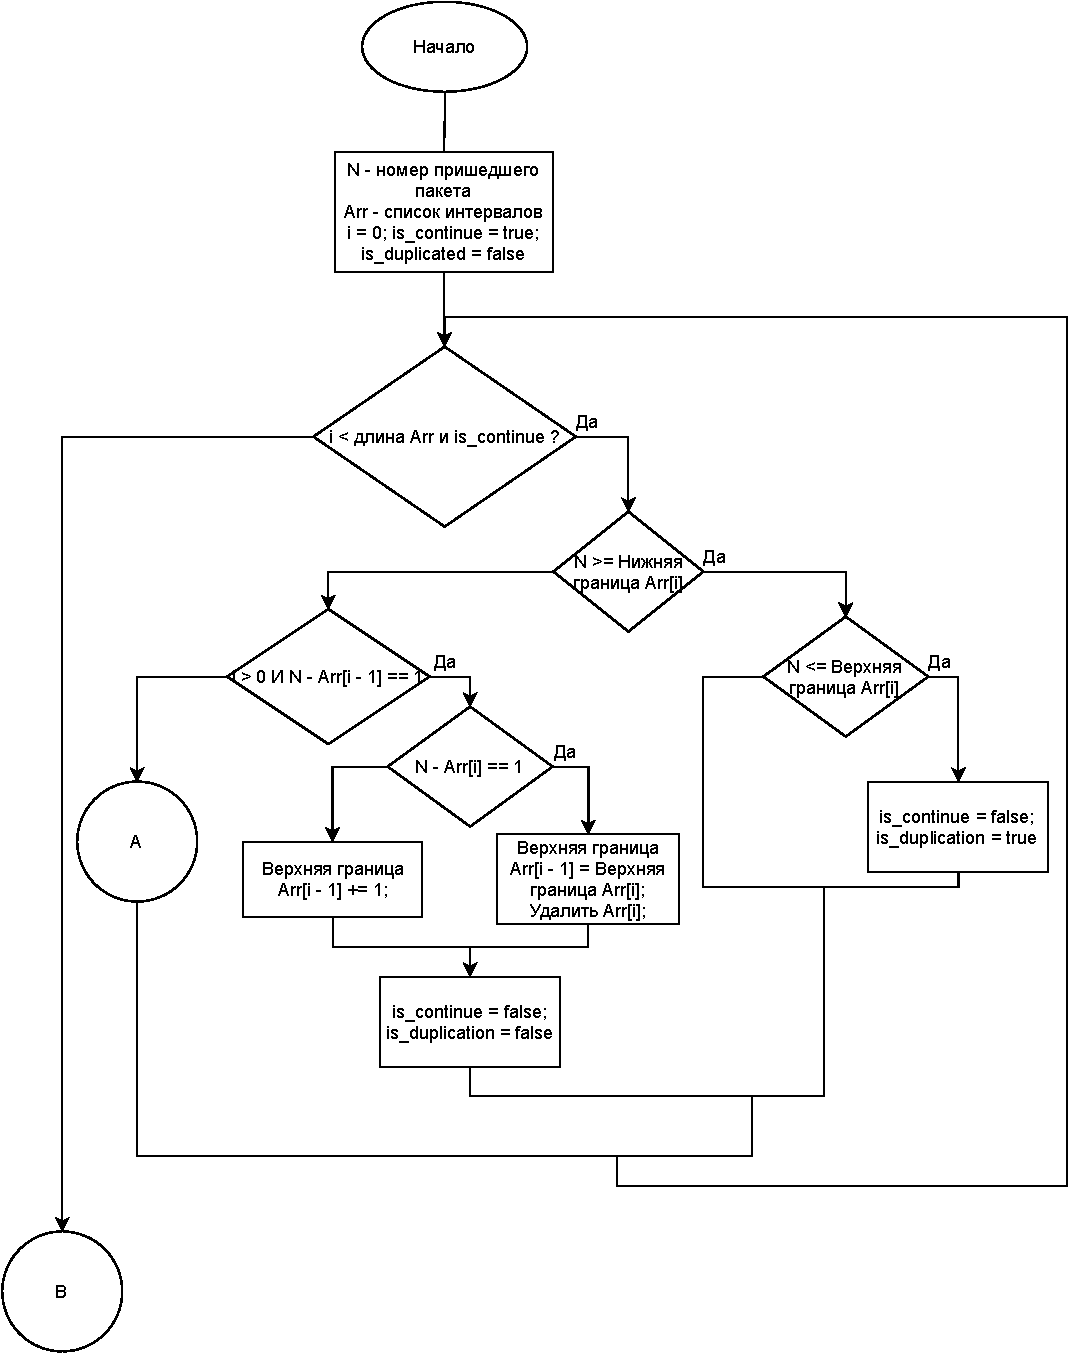
\includegraphics[scale=0.9]{check1.pdf}
	\caption{Первая часть проверки и добавления}
	\label{check1}
\end{figure}

\begin{figure}[H]
	\centering
	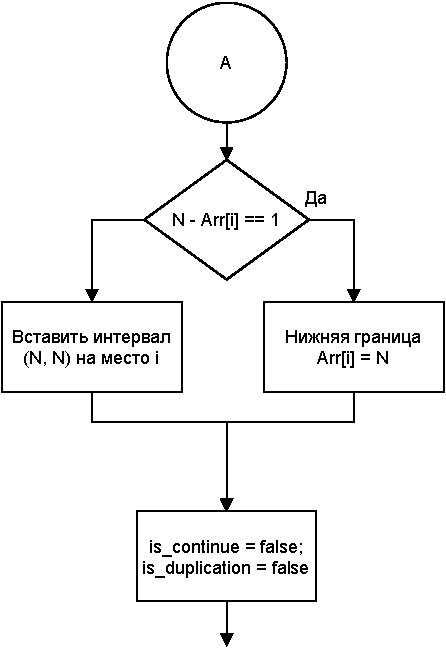
\includegraphics[scale=1]{check2.pdf}
	\caption{Вторая часть проверки и добавления}
	\label{check2}
\end{figure}

\begin{figure}[H]
	\centering
	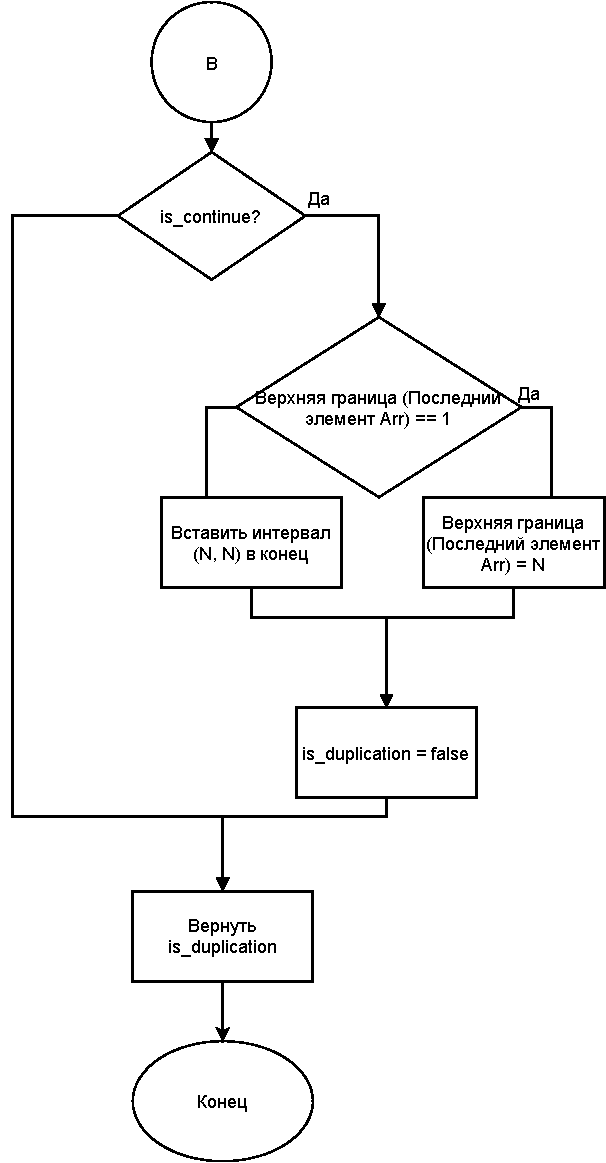
\includegraphics[scale=1]{check3.pdf}
	\caption{Третья часть проверки и добавления}
	\label{check3}
\end{figure}

Для корректного отбрасывания накопленных интервалов необходимо ввести правило отбрасывания отмлеживания устаревших пакетов. По аналогии с TCP логично ввести окно, но, в отличии от TCP можно отказаться от его динамичности. Таким образом вводится статическое окно, всегда содержащее интервал в N пакетов. \\
\indent Из вышеизложенного алгоритма сразу вытекает крайний случай. Если на стороне клиента произошел сбой, то нумерация отправленных пакетов начнется сначала и, если они уже были приняты в предвдущей сессии, то они начнут отбрасываться, пока номер пакета не превысит номер последнего принятого пакета. \\ 
\indent Для решения этой проблемы стоит ввести идентификатор начала передачи пакетов, по которому будет происходить обнуление отслеживаемых интервалов. И для надежной его передачи --- пакет подтверждение. На рисунке \ref{catch} представлена общая схема обработки пакета на принимающей стороне, а на рисунке \ref{send} --- со стороны отправки.
\begin{figure}[H]
	\centering
	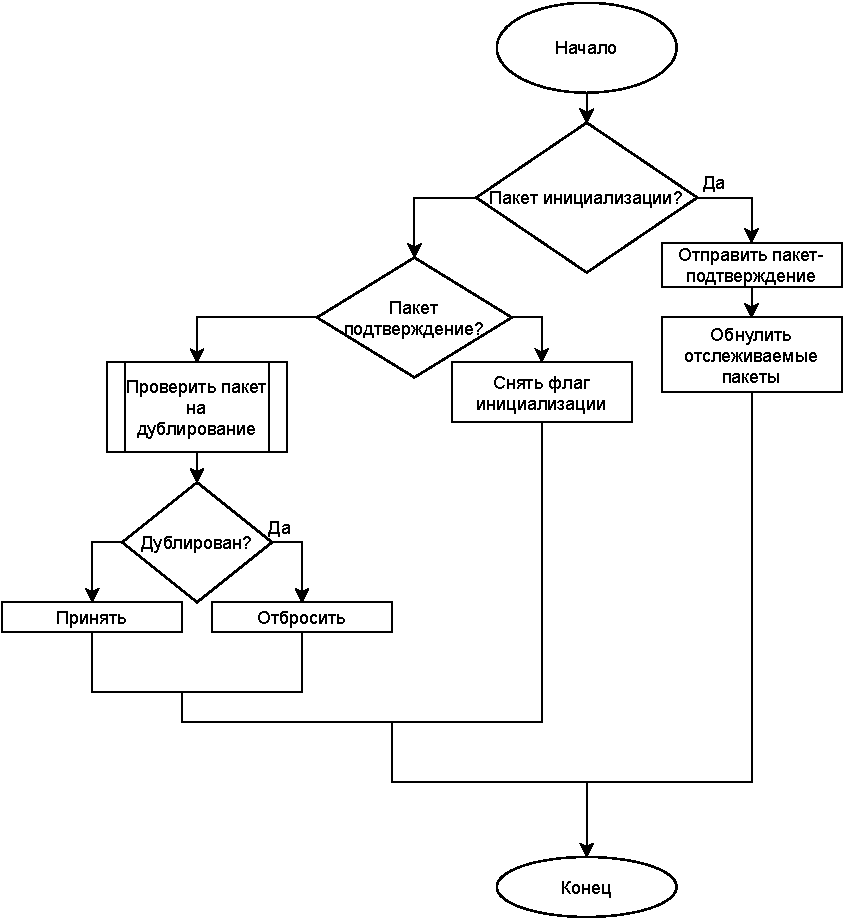
\includegraphics[scale=1]{catch.pdf}
	\caption{Алгоритм получения пакеты}
	\label{catch}
\end{figure}

\begin{figure}[H]
	\centering
	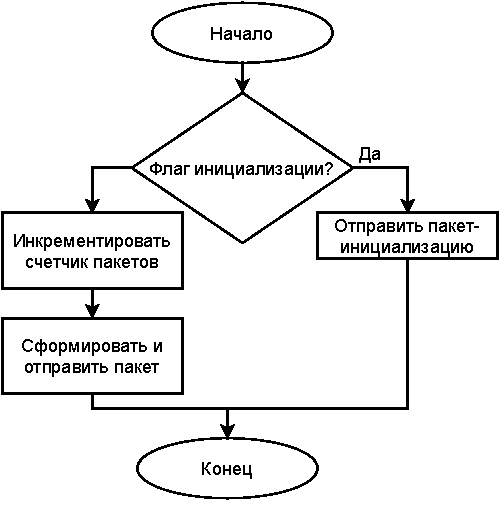
\includegraphics[scale=1]{send.pdf}
	\caption{Алгоритм отправки пакета}
	\label{send}
\end{figure}

\indent Для реализации передачи типа пакета необходимо добавить соответствующее поле в заголовок пакета.
\subsection{Вывод}
В конструкторской части был описан протокол, спроектированы основные алгоритмы. 

\clearpage
\section{Технологический раздел}
\subsection{Выбор языка и среды программирования}
В качестве языка программирования для реализации поставленной
задачи был выбран язык Rust\cite{rust} --- мультипарадигмальный компилируемый язык программирования общего назначения, часто используется для системного программирования. Средой разработки был выбран текстовый редактор Visual Studio Code\cite{vscode}.

\subsection{Описание основных структур}
Для реализации хранения номяров принятых пакетов была написана структура filter. На листинге \ref{filter} приведена эта структура.

\begin{lstlisting}[caption=filter, label={filter}]
pub struct Filter {
	state: bool,
	window_size: usize,
	received_packets: Vec<(usize, usize)>,
}
\end{lstlisting}
Описание полей структуры:
\begin{itemize}
	\item state --- состояние активности фильтра;
	\item window\_size --- размер окна;
	\item received\_packets --- список хранения интервалов.
\end{itemize}

Заголовок пакета был реализован с помощью следующих структур:
\begin{lstlisting}[caption=Заголовок пакета, label={filter}]
pub enum PacketKind {
	Init,	
	Data,
	Ack,
}

pub struct Header {
	index: u32,
	payload_len: u32,
	kind: PacketKind,
}

\end{lstlisting}

\subsection{Реализация}
На основе алгоритма из конструкторской части была написана функция проверки дублирования пакета. На листинге \ref{dup} представлена эта функция.
\begin{lstlisting}[caption=Проверка на дублирование, label=dup]
 fn check_duplicate(&mut self, i: usize) -> bool {
	let len = self.received_packets.len();
	for c in 0..end {
		if i >= self.received_packets[c].0 {
			if i <= self.received_packets[c].1 {
				return true;
			}
			continue;
		} else if (c != 0) && ((i - self.received_packets[c - 1].1) == 1) {
			if (self.received_packets[c].0 - i) == 1 {
				self.received_packets[c - 1].1 = self.received_packets[c].1;
				self.received_packets.remove(c);
			} else {
				self.received_packets[c - 1].1 = i;
			}
			return false;
		} else if (self.received_packets[c].0 - i) == 1 {
			self.received_packets[c].0 = i;
			return false;
		}
		self.received_packets.insert(c, (i, i));
		return false;
	}
	if i - self.received_packets[len - 1].1 == 1 {
		self.received_packets[len - 1].1 = i;
	} else {
		self.received_packets.insert(len, (i, i));
	}
	false
}
\end{lstlisting}
На основе алгоритма из конструкторской части была написана функция обработки получения пакета. На листинге \ref{get} представлена часть этой функции.
\begin{lstlisting}[caption=Получение пакета, label=get]
 if packet.is_init() {
	dup_filter.init();
} else if !dup_filter.is_duplicate(packet.index() as usize) {
	// обработка
}
\end{lstlisting}


\subsection{Вывод}
В технологической части были реализаны спроектированные функции.

\clearpage
\section{Технологическая часть}
Для тестирования реализованного протокола были выбраны следующие средства:
\begin{itemize}
	\item iperf3 --- утилита для генерации трафика\cite{iperf3};
	\item netem --- утилита для изменения параметров канала\cite{netem}.
\end{itemize}

На рисунке \ref{setnetem} показана настройка утилиты netem. В данном случае произведена настройка канала на 20\% дублирования пакетов.
\begin{figure}[H]
	\centering
	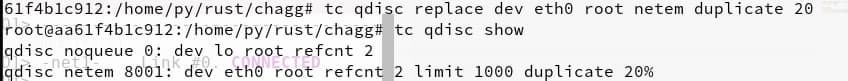
\includegraphics[scale=0.7]{setnetem.jpg}
	\caption{Настройка netem}
	\label{setnetem}
\end{figure}

На рисунке \ref{resoff} показан результат работы утилиты iperf3 при выключенной дедупликации. Как видно из отчета работы, примерно 20\% пакетов приходят вне очереди, что в данном случае показывает приход дублированных пакетов.
\begin{figure}[H]
	\centering
	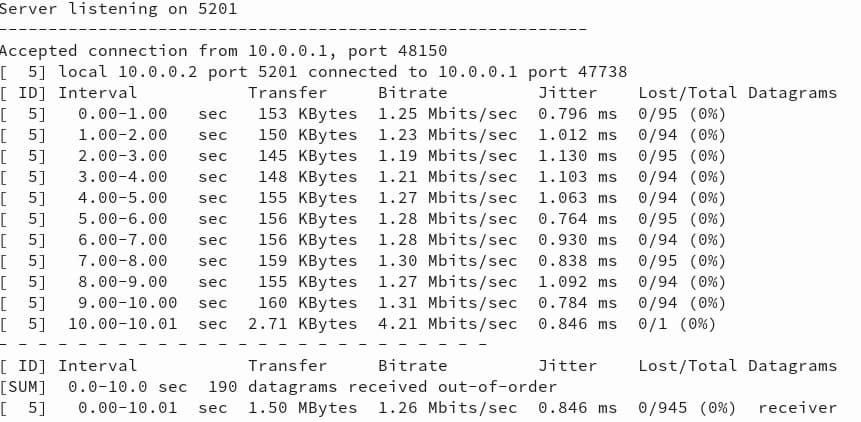
\includegraphics[scale=0.7]{resoff.jpg}
	\caption{Iperf3 без дедупликации}
	\label{resoff}
\end{figure}

На рисунке \ref{reson} показан результат работы утилиты iperf3 при включенной дедупликации. Как видно из отчета работы, дублирование отсутствует, что значит, что реализованный алгоритм работает.
\begin{figure}[H]
	\centering
	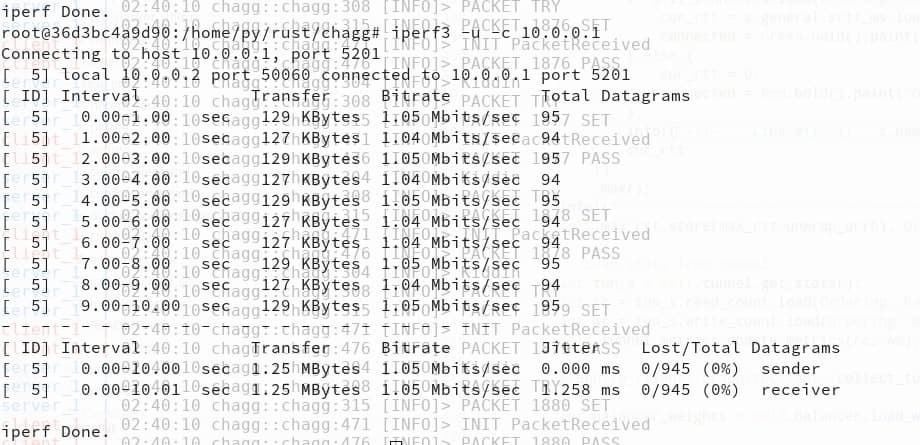
\includegraphics[scale=0.7]{reson.jpg}
	\caption{Iperf3 со дедупликацией}
	\label{reson}
\end{figure}

\clearpage
\section*{Заключение}
\addcontentsline{toc}{section}{Заключение}
В процессе выполнения курсовой работы были изучены основы работы протоколов UDP и TCP, проанализирована предметная область. Был спроектирован, реализован и протестирован протокол, отбрасывающий дубликаты пакетов. \\
\indent Цель работы достигнута, все задачи выполнены. 
\clearpage
\begin{thebibliography}{9}
	\addcontentsline{toc}{section}{Литература}
	\bibitem{quality} Lossrate and RTT inspecting. [Электронный ресурс] URL: https://netbeez.net/blog/packet-loss-round-trip-time-tcp/ (дата обращения: 31.12.2021)
	\bibitem{rfc768} UDP. RFC768. [Электронный ресурс] URL: https://datatracker.ietf.org/doc/html/rfc768 (дата обращения: 31.12.2021)
	\bibitem{rfc793} UDP. RFC768. [Электронный ресурс] URL: https://datatracker.ietf.org/doc/html/rfc793 (дата обращения: 31.12.2021)
	\bibitem{tcpheader} Header TCP. [Электронный ресурс] URL: https://networkguru.ru/protokol-transportnogo-urovnia-tcp-chto-nuzhno-znat/ (дата обращения: 31.12.2021)
	\bibitem{rust} Rust. [Электронный ресурс] URL: https://www.rust-lang.org/ (дата обращения: 31.12.2021)
	\bibitem{vscode} VS Code. [Электронный ресурс] URL: https://code.visualstudio.com/ (дата обращения: 31.12.2021)
	\bibitem{netem} Netem. [Электронный ресурс] URL: https://man7.org/linux/man-pages/man8/tc-netem.8.html (дата обращения: 31.12.2021)
	\bibitem{iperf3} Iperf3. [Электронный ресурс] URL: https://github.com/esnet/iperf (дата обращения: 31.12.2021)
	
\end{thebibliography}


\end{document}




